\documentclass[]{scrartcl}
\usepackage{lmodern}
\usepackage{amssymb,amsmath}
\usepackage{ifxetex,ifluatex}
\usepackage{fixltx2e} % provides \textsubscript
\ifnum 0\ifxetex 1\fi\ifluatex 1\fi=0 % if pdftex
  \usepackage[T1]{fontenc}
  \usepackage[utf8]{inputenc}
\else % if luatex or xelatex
  \ifxetex
    \usepackage{mathspec}
  \else
    \usepackage{fontspec}
  \fi
  \defaultfontfeatures{Ligatures=TeX,Scale=MatchLowercase}
\fi
% use upquote if available, for straight quotes in verbatim environments
\IfFileExists{upquote.sty}{\usepackage{upquote}}{}
% use microtype if available
\IfFileExists{microtype.sty}{%
\usepackage{microtype}
\UseMicrotypeSet[protrusion]{basicmath} % disable protrusion for tt fonts
}{}
\usepackage{hyperref}
\hypersetup{unicode=true,
            pdftitle={Angabe},
            pdfauthor={Team\ldots{}},
            pdfborder={0 0 0},
            breaklinks=true}
\urlstyle{same}  % don't use monospace font for urls
\IfFileExists{parskip.sty}{%
\usepackage{parskip}
}{% else
\setlength{\parindent}{0pt}
\setlength{\parskip}{6pt plus 2pt minus 1pt}
}
\setlength{\emergencystretch}{3em}  % prevent overfull lines
\providecommand{\tightlist}{%
  \setlength{\itemsep}{0pt}\setlength{\parskip}{0pt}}
\setcounter{secnumdepth}{5}
% Redefines (sub)paragraphs to behave more like sections
\ifx\paragraph\undefined\else
\let\oldparagraph\paragraph
\renewcommand{\paragraph}[1]{\oldparagraph{#1}\mbox{}}
\fi
\ifx\subparagraph\undefined\else
\let\oldsubparagraph\subparagraph
\renewcommand{\subparagraph}[1]{\oldsubparagraph{#1}\mbox{}}
\fi

\usepackage{graphicx}
\usepackage{array}
\usepackage{ragged2e}
\usepackage[section]{placeins}
\makeatletter
\AtBeginDocument{%
  \expandafter\renewcommand\expandafter\subsection\expandafter{%
    \expandafter\@fb@secFB\subsection
  }%
}
\makeatother
 
\title{Angabe 1}
\providecommand{\subtitle}[1]{}
\subtitle{Untertitel}
\author{Daniel Graf, Dimitrie Diez, Arne Schöntag, Peter Müller}
\date{}

\begin{document}
\maketitle


\tableofcontents

\section{Einführung}

% Problem -> Motivation

\section{Messexperiment}

Das Messexperiment wurde am $05.04.2017$ im Lichthof der Hochschule München (Lothstraße 64) durchgeführt. Es nahmen $22$ Probanden im Alter von $20-29$ Jahren teil. Das Experiment bestand aus drei Teilen. 

Zunächst wurde die Wunschgeschwindigkeit in der Ebene gemessen. Hierfür ging jeder Proband eine markierte Strecke von $27,3m$ ab und stoppte die hierfür benötigte Zeit. Anschließend wurde dieser Vorgang zweimal wiederholt und die entsprechende Rundennummer vermerkt. Im zweiten Teil erfolgte die Messung der benötigten Zeit für einen Treppenaufstieg. Die Treppenlänge betrug $9m$. Jeder Proband führte den Vorgang dreimal durch und vermerkte die benötigte Zeit und die entsprechende Rundennummer. Analog hierzu wurde im dritten Teil des Experiments die Zeit beim Treppenabstieg gemessen. 

Neben den gemessenen Zeiten in jeder Runde, dem Alter und der Körpergröße ist auch das Geschlecht jedes Probanden bekannt. Weitere Informationen sind in der beiliegenden Versuchsbeschreibung "Choreographie\_Treppengeschwindigkeit\_2017" aufgeführt. In den folgenden Kapiteln erfolgt die Auswertung der ermittelten Messwerte.

\section{Überprüfung auf Normalverteilung}

\section{Lineare Regression}

Um Hinweise auf einen möglichen Zusammenhang der Treppengeschwindigkeit mit weiteren durch das Messexperiment ermittelten Größen zu finden, wird eine lineare 
Regression angewandt.

Die hier betrachteten Größen sind Wunschgeschwindigkeit (in der Ebene),
Körpergröße und Rundennummer. Es wird gesondert die Treppengeschwindigkeit aufwärts und abwärts betrachtet.
Zunächst wird nur auf eine Abhängigkeit überprüft, danach die Abhängigkeit von mehreren kombinierten Größen. Die Zusammenhänge werden bezüglich ihrer Plausibilität bewertet.

\subsection{Prüfung auf eine einfache Abhängigkeit}

Hier werden sechs Gleichungen mittels linearer Regression ermittelt: 

\[v_{auf}(v_{ebene}) = \beta_0 + \beta_1 v_{ebene}\]
\[v_{ab}(v_{ebene}) = \beta_0 + \beta_1 v_{ebene}\]

\[v_{auf}(groesse) = \beta_0 + \beta_1 groesse\]
\[v_{ab}(groesse) = \beta_0 + \beta_1 groesse\]

\[v_{auf}(runde) = \beta_0 + \beta_1 runde\]
\[v_{ab}(runde) = \beta_0 + \beta_1 runde\]

\subsubsection{Wunschgeschwindigkeit in der Ebene}

Für die Abhängigkeit Wunschgeschwindigkeit in der Ebene wurde 
der Zusammenhang wie in den Formeln für die Treppengeschwindigkeit aufwärts (\ref{eq:auf-ebene}) und abwärts (\ref{eq:ab-ebene}) ermittelt. 

\begin{equation} \label{eq:auf-ebene}
	v_{auf}(v_{ebene}) = 0.294389 + 0.393467 v_{ebene}
\end{equation}
\begin{equation} \label{eq:ab-ebene}
	v_{ab}(v_{ebene}) = 0.440848 + 0.478525 v_{ebene}
\end{equation}

Beide Steigungen sind positiv. Hat ein Proband eine schnellere Wunschgeschwindigkeit in der Ebene verhält er sich auch schneller auf 
der Treppe. Die Abbildungen \ref{fig:auf-ebene} und \ref{fig:ab-ebene}
stellen dies grafisch dar. 

\begin{figure} \centering 
	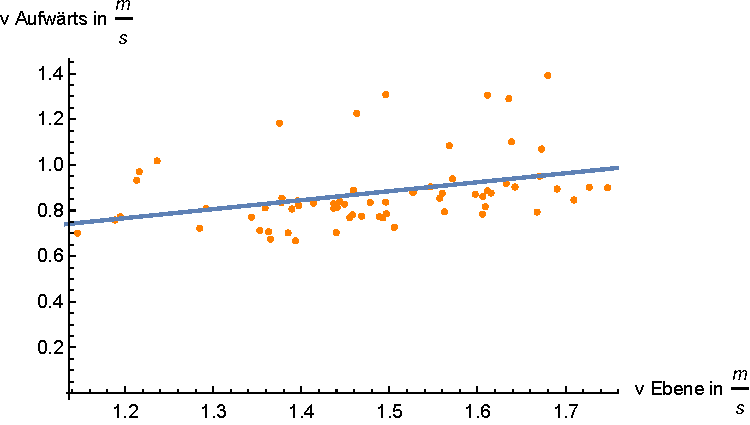
\includegraphics[]{abbildungen/regression/2017/auf-ebene.pdf}
	\[\begin{array}{l|llll}
 \text{} & \text{Estimate} & \text{Standard Error} & \text{t-Statistic} & \text{P-Value} \\
\hline
 1 & 0.506746 & 0.0900029 & 5.63033 & \text{2.603647901106944$\grave{ }$*${}^{\wedge}$-6} \\
 \text{vEbene} & 0.168071 & 0.0588553 & 2.85567 & 0.00727064 \\
\end{array}\]


	\caption{Abhängigkeit Wunschgeschwindigkeit in der Ebene zur Treppengeschwindigkeit aufwärts. Messdaten (orange) mit ermittelter Regressionsgerade (blau). \label{fig:auf-ebene}}
\end{figure}

\begin{figure} \centering 
	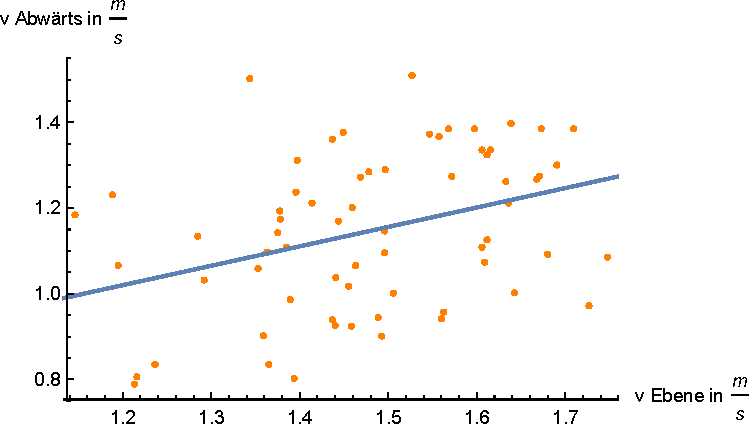
\includegraphics[]{abbildungen/regression/2017/ab-ebene.pdf}
	\[\begin{array}{l|llll}
 \text{} & \text{Estimate} & \text{Standard Error} & \text{t-Statistic} & \text{P-Value} \\
\hline
 1 & 0.440848 & 0.213068 & 2.06904 & 0.0428577 \\
 \text{vEbene} & 0.478525 & 0.142985 & 3.34668 & 0.00141579 \\
\end{array}\]


	\caption{Abhängigkeit Wunschgeschwindigkeit in der Ebene zur Treppengeschwindigkeit abwärts. Messdaten (orange) mit ermittelter Regressionsgerade (blau). \label{fig:ab-ebene}}
\end{figure}

In Abbildung \ref{fig:auf-ebene} sind wieder
deutlich die schon in der Betrachtung zur Normalverteilung erwähnten Ausreißer zu erkennen. Deshalb wurde die lineare Regression für den gefilterten Messdatensatz (nur Datensätze ohne Bemerkung) durchgeführt. Es ergeben sich neue Formeln für die Treppengeschwindigkeit aufwärts (\ref{eq:ohne-auf-ebene}) und abwärts (\ref{eq:ohne-ab-ebene}). Dazu gehören Abbildungen \ref{fig:ohne-auf-ebene} und \ref{fig:ohne-ab-ebene}. Die Ausreißer wurden in der Regression hier nicht verwendet, sind aber hervorgehoben eingezeichnet. Bei der Treppengeschwindigkeit sind es deutlich mehr Ausreißer und sie fallen alle in den schnelleren Bereich. Die Regressionsgerade für die Daten ohne Ausreißer liegt dementsprechend 
etwas weiter unter (langsamer) im Vergleich zu Abbildung \ref{fig:auf-ebene}. Bei Abbildung \ref{fig:ohne-ab-ebene} sind es nur 
vier Ausreißer. Sie sind auch stärker gestreut. Die Regressionsgerade für den Zusammenhang zur Geschwindigkeit abwärts wird nicht besonders von dem Weglassen der Ausreißer beeinflusst. Die Ausreißer werden in den weiteren Regressionen nicht genauer betrachtet. Alle Abbildungen und Plausibilisierungstests dazu sind aber als Dateien angelegt.

\begin{equation} \label{eq:ohne-auf-ebene}
	v'_{auf}(v_{ebene}) = 0.332577 +0.325892 v_{ebene}
\end{equation}
\begin{equation} \label{eq:ohne-ab-ebene}
	v'_{ab}(v_{ebene}) = 0.475883\, +0.453419 v_{ebene}
\end{equation}

\begin{figure} \centering 
	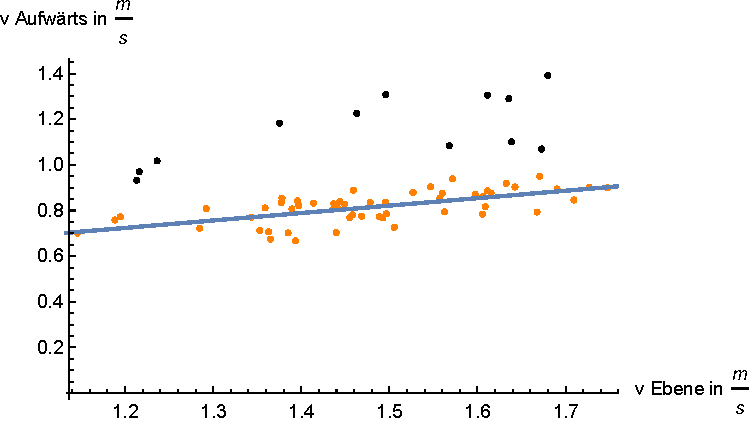
\includegraphics[]{abbildungen/regression/2017/ohneausreisser/auf-ebene.pdf}
	\caption{Abhängigkeit Wunschgeschwindigkeit in der Ebene zur Treppengeschwindigkeit aufwärts. Gefilterte Messdaten (orange) und Ausreißer (schwarz) mit ermittelter Regressionsgerade (blau). \label{fig:ohne-auf-ebene}}
\end{figure}

\begin{figure} \centering 
	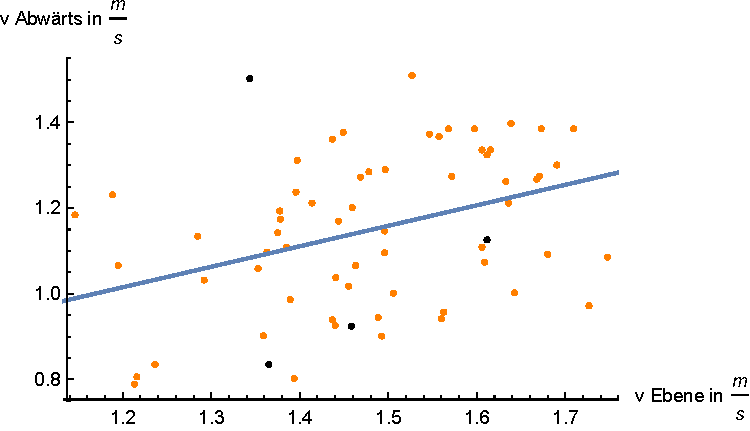
\includegraphics[]{abbildungen/regression/2017/ohneausreisser/ab-ebene.pdf}
	\caption{Abhängigkeit Wunschgeschwindigkeit in der Ebene zur Treppengeschwindigkeit abwärts. Gefilterte Messdaten (orange) und Ausreißer (schwarz) mit ermittelter Regressionsgerade (blau).
	\label{fig:ohne-ab-ebene}}
\end{figure}

Für die Plausibilisierung der Regression wird die Nullhypothese 
$H_0: \beta_1 = 0$ aufgestellt. Signifikanzniveau $\alpha = 0.05$.
Die Ergebnisse des Tests sind in Abbildung \ref{fig:auf-ebene} zu sehen.
Signifikanz liegt vor, weil $p < \alpha$. Man verwirft die
Nullhypothese. Kein Einfluss von $v_{ebene}$ auf $v_{auf}$ wäre unplausibel, wenn auch nicht ausgeschlossen.

Die Nullhypothese und das Signifikanzniveau sind für alle folgenden Regressionen gleich. Die Ergebnisse für den Abstieg sind in \ref{fig:auf-ebene} zu sehen.
Signifikanz liegt vor, weil $p < \alpha$. Man verwirft die
Nullhypothese. Kein Einfluss von $v_{ebene}$ auf $v_{ab}$ wäre unplausibel, wenn auch nicht ausgeschlossen.

\subsubsection{Körpergröße}

Für die Abhängigkeit Körpergröße wurde 
der Zusammenhang (\ref{eq:auf-groesse}) und (\ref{eq:ab-groesse}) ermittelt.

\begin{equation} \label{eq:auf-groesse}
	v_{auf}(groesse) = 0.133389 + 0.00419914 groesse
\end{equation}
\begin{equation} \label{eq:ab-groesse}
	v_{ab}(groesse) = 1.59558 - 0.00253145 groesse
\end{equation}

In den Abbildungen \ref{fig:auf-groesse} und \ref{fig:ab-groesse} ist 
zu sehen, dass nach dem Modell größere Personen leicht schneller Treppen besteigen, aber beim herabsteigen etwas langsamer als kleinere
Personen sind. 

\begin{figure} \centering 
	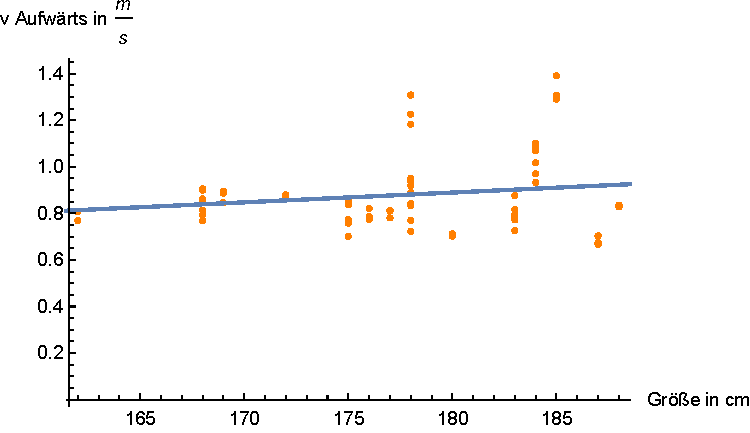
\includegraphics[]{abbildungen/regression/2017/auf-groesse.pdf}
	\[\begin{array}{l|llll}
 \text{} & \text{Estimate} & \text{Standard Error} & \text{t-Statistic} & \text{P-Value} \\
\hline
 1 & 1.42188 & 0.660147 & 2.15388 & 0.0335816 \\
 \text{gr{\" o}{\ss}e} & -0.00301832 & 0.0037105 & -0.813455 & 0.417834 \\
\end{array}\]


	\caption{Abhängigkeit Körpergröße zur Treppengeschwindigkeit aufwärts. Messdaten (orange) mit ermittelter Regressionsgerade (blau). \label{fig:auf-groesse}}
\end{figure}

\begin{figure} \centering 
	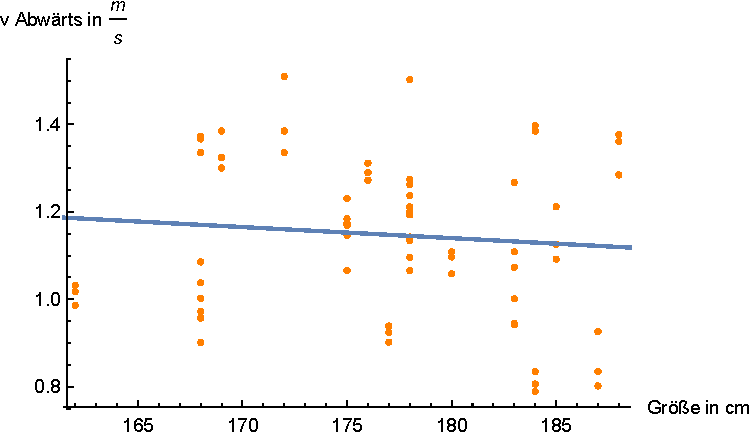
\includegraphics[]{abbildungen/regression/2017/ab-groesse.pdf}
	\[\begin{array}{l|llll}
 \text{} & \text{Estimate} & \text{Standard Error} & \text{t-Statistic} & \text{P-Value} \\
\hline
 1 & 1.59558 & 0.582855 & 2.73753 & 0.00800578 \\
 \text{gr{\" o}{\ss}e} & -0.00253145 & 0.00328881 & -0.769715 & 0.444301 \\
\end{array}\]


	\caption{Abhängigkeit Körpergröße zur Treppengeschwindigkeit abwärts. Messdaten (orange) mit ermittelter Regressionsgerade (blau). \label{fig:ab-groesse}}
\end{figure}

Ergebnisse der Plausibilisierung für den Aufstieg 
(Abbildung \ref{fig:auf-groesse}):
Signifikanz liegt nicht vor, weil $p > \alpha$. Man nimmt die
Nullhypothese an. Kein Einfluss von $groesse$ auf $v_{auf}$ ist plausibel.

Ergebnisse der Plausibilisierung für den Abstieg
(Abbildung \ref{fig:ab-groesse}):
Signifikanz liegt vor, weil $p > \alpha$. Man nimmt die
Nullhypothese an. Kein Einfluss von $groesse$ auf $v_{ab}$ ist plausibel.


\subsubsection{Rundennummer}


Für die Abhängigkeit Rundennummer wurde 
der Zusammenhang (\ref{eq:auf-runde}) und (\ref{eq:ab-runde}) ermittelt.

\begin{equation} \label{eq:auf-runde}
v_{auf}(runde) = 0.890435 - 0.00670795 runde
\end{equation}
\begin{equation} \label{eq:ab-runde}
v_{ab}(runde) = 1.14614\, +0.000574582 runde
\end{equation}

In den Abbildungen \ref{fig:auf-runde} und \ref{fig:ab-runde} ist 
zu sehen, dass sich nach dem Modell die Treppengeschwindigkeit bei Änderung der Runde fast nicht ändert. 

\begin{figure} \centering 
	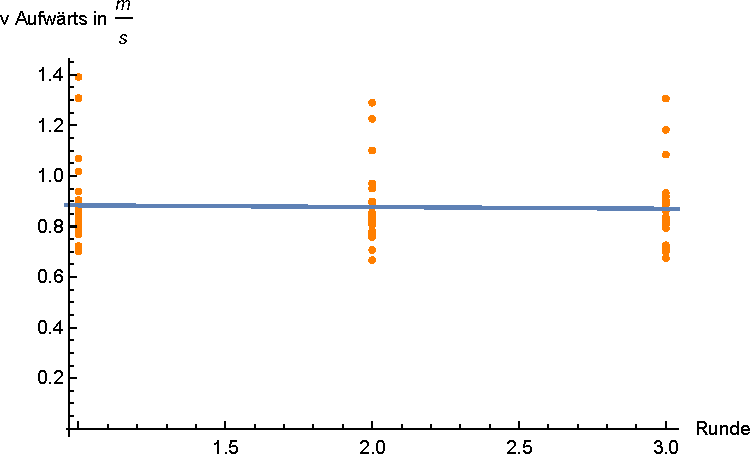
\includegraphics[]{abbildungen/regression/2017/auf-runde.pdf}
	\[\begin{array}{l|llll}
 \text{} & \text{Estimate} & \text{Standard Error} & \text{t-Statistic} & \text{P-Value} \\
\hline
 1 & 0.94804 & 0.2081 & 4.55569 & 0.0000551454 \\
 \text{runde} & -0.0241206 & 0.0963317 & -0.250391 & 0.80367 \\
\end{array}\]


	\caption{Abhängigkeit Rundennummer zur Treppengeschwindigkeit aufwärts. Messdaten (orange) mit ermittelter Regressionsgerade (blau). \label{fig:auf-runde}}
\end{figure}

\begin{figure} \centering 
	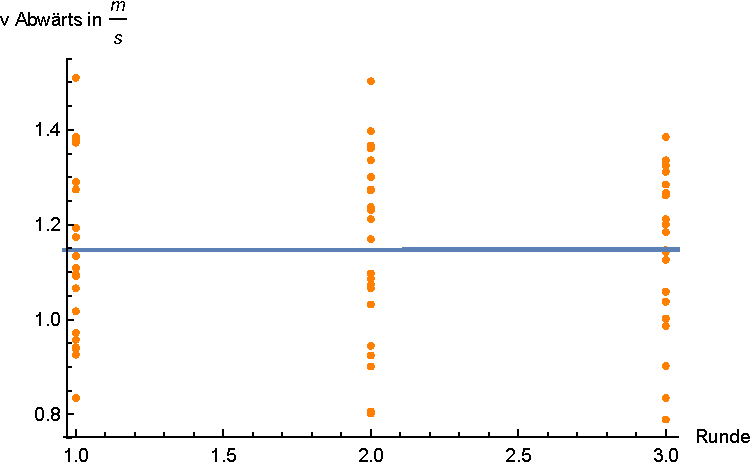
\includegraphics[]{abbildungen/regression/2017/ab-runde.pdf}
	\[\begin{array}{l|llll}
 \text{} & \text{Estimate} & \text{Standard Error} & \text{t-Statistic} & \text{P-Value} \\
\hline
 1 & 0.859522 & 0.0289618 & 29.6777 & \text{6.817362585804904$\grave{ }$*${}^{\wedge}$-26} \\
 \text{runde} & 0.00475595 & 0.0134067 & 0.354744 & 0.724973 \\
\end{array}\]


	\caption{Abhängigkeit Rundennummer zur Treppengeschwindigkeit abwärts. Messdaten (orange) mit ermittelter Regressionsgerade (blau). \label{fig:ab-runde}}
\end{figure}

Ergebnisse der Plausibilisierung für den Aufstieg
(Abbildung \ref{fig:auf-runde}):
Signifikanz liegt nicht vor, weil $p > \alpha$. Man nimmt die
Nullhypothese an. Kein Einfluss von $runde$ auf $v_{auf}$ ist plausibel.

Ergebnisse der Plausibilisierung für den Abstieg
(Abbildung \ref{fig:ab-runde}):
Signifikanz liegt vor, weil $p > \alpha$. Man nimmt die
Nullhypothese an. Kein Einfluss von $runde$ auf $v_{ab}$ ist plausibel.

\subsection{Mehrere Abhängigkeiten}

Hier werden weitere vier lineare Gleichungen mit mehreren Parametern ermittelt.

\[v_{auf}(v_{ebene}, groesse) = \beta_0 + \beta_1 v_{ebene} + \beta_2 groesse\]
\[v_{ab}(v_{ebene}, groesse) = \beta_0 + \beta_1 v_{ebene} + \beta_2 groesse\]

\[v_{auf}(v_{ebene}, groesse, runde) = \beta_0 + \beta_1 v_{ebene} + \beta_2 groesse + \beta_3 groesse\]
\[v_{ab}(v_{ebene}, groesse, runde) = \beta_0 + \beta_1 v_{ebene} + \beta_2 groesse + \beta_3 runde\]

\subsubsection{Ebenengeschwindigkeit und Größe}

Für die Abhängigkeiten Wunschgeschwindigkeit in der Ebene und Körpergröße wurde 
der Zusammenhang (\ref{eq:auf-runde}) und (\ref{eq:ab-runde}) ermittelt.

\begin{figure} \centering 
	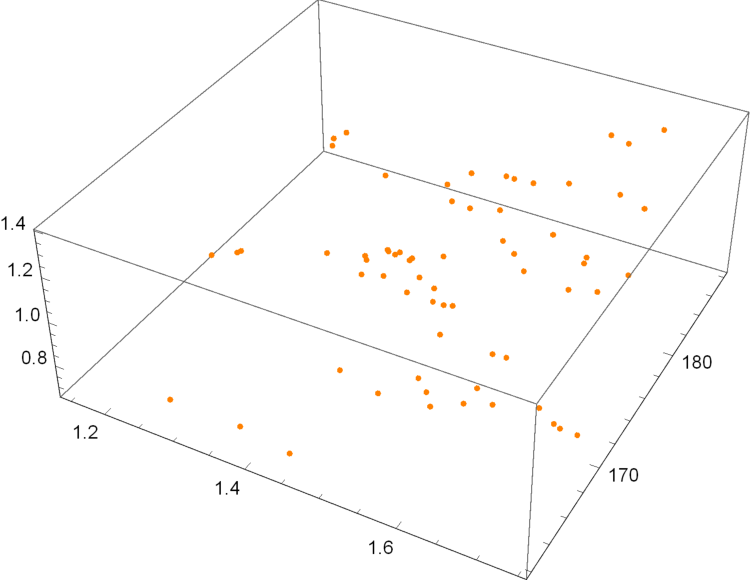
\includegraphics[]{abbildungen/regression/2017/auf-ebene-groesse.pdf}
	\[\begin{array}{l|llll}
 \text{} & \text{Estimate} & \text{Standard Error} & \text{t-Statistic} & \text{P-Value} \\
\hline
 1 & 1.0165 & 0.140132 & 7.25384 & \text{1.5820003769083974$\grave{ }$*${}^{\wedge}$-10} \\
 \text{vEbene} & 0.199894 & 0.0433176 & 4.61461 & 0.0000134806 \\
 \text{gr{\" o}{\ss}e} & -0.00294506 & 0.000643082 & -4.5796 & 0.0000154292 \\
\end{array}\]


	\caption{Abhängigkeiten Ebenengeschwindigkeit und Größe zur Treppengeschwindigkeit aufwärts. Messdaten (orange) mit ermittelter Regressionsebene (blau). \label{fig:auf-ebene-groesse}}
\end{figure}

\begin{figure} \centering 
	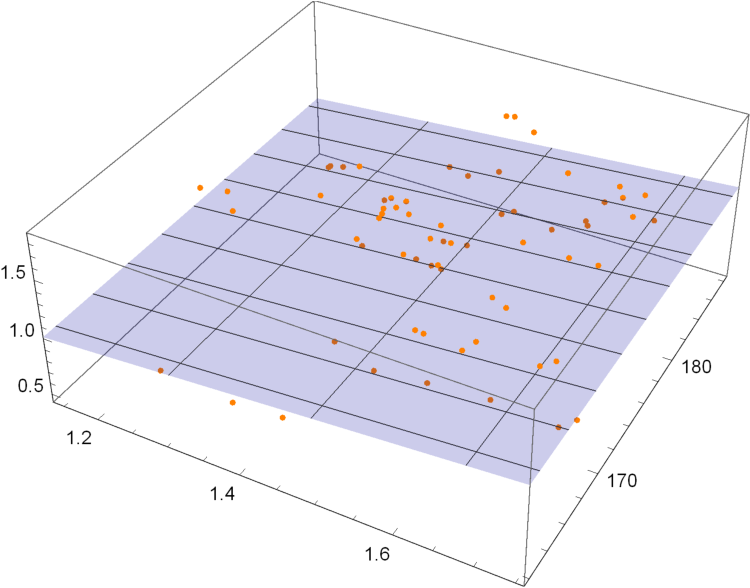
\includegraphics[]{abbildungen/regression/2017/ab-ebene-groesse.pdf}
	\[\begin{array}{l|llll}
 \text{} & \text{Estimate} & \text{Standard Error} & \text{t-Statistic} & \text{P-Value} \\
\hline
 1 & 0.701775 & 0.543236 & 1.29184 & 0.199331 \\
 \text{vEbene} & 0.696676 & 0.127843 & 5.44946 & \text{3.523565756565165$\grave{ }$*${}^{\wedge}$-7} \\
 \text{gr{\" o}{\ss}e} & -0.00382545 & 0.00268911 & -1.42257 & 0.157912 \\
\end{array}\]


	\caption{Abhängigkeiten Ebenengeschwindigkeit und Größe zur Treppengeschwindigkeit abwärts. Messdaten (orange) mit ermittelter Regressionsebene (blau). \label{fig:ab-ebene-groesse}}
\end{figure}

\subsubsection{Ebenengeschwindigkeit, Größe und Rundennummer}

Für die Abhängigkeiten Wunschgeschwindigkeit in der Ebene ,Körpergröße und Rundennummer wurde 
der Zusammenhang (\ref{eq:auf-runde}) und (\ref{eq:ab-runde}) ermittelt.

\begin{figure} \centering 
	\[\begin{array}{l|llll}
 \text{} & \text{Estimate} & \text{Standard Error} & \text{t-Statistic} & \text{P-Value} \\
\hline
 1 & -1.06201 & 0.581909 & -1.82505 & 0.0709498 \\
 \text{runde} & -0.0035349 & 0.0291243 & -0.121373 & 0.903637 \\
 \text{vEbene} & 1.18933 & 0.136075 & 8.74028 & \text{5.287415408789427$\grave{ }$*${}^{\wedge}$-14} \\
 \text{gr{\" o}{\ss}e} & 0.000853656 & 0.00286026 & 0.298454 & 0.76597 \\
\end{array}\]


	\caption{Abhängigkeiten Ebenengeschwindigkeit, Größe und Runde zur Treppengeschwindigkeit aufwärts.
	\label{fig:auf-ebene-groesse}}
\end{figure}

\begin{figure} \centering 
	\[\begin{array}{l|llll}
 \text{} & \text{Estimate} & \text{Standard Error} & \text{t-Statistic} & \text{P-Value} \\
\hline
 1 & -0.893281 & 0.654301 & -1.36525 & 0.180888 \\
 \text{runde} & 0.0153806 & 0.0381571 & 0.403085 & 0.689337 \\
 \text{vEbene} & 1.27163 & 0.152749 & 8.32501 & \text{8.139962234647669$\grave{ }$*${}^{\wedge}$-10} \\
 \text{gr{\" o}{\ss}e} & -0.00100623 & 0.00306762 & -0.328015 & 0.744854 \\
\end{array}\]


	\caption{Abhängigkeiten Ebenengeschwindigkeit, Größe und Runde zur Treppengeschwindigkeit abwärts.
	\label{fig:ab-ebene-groesse}}
\end{figure}

\subsection{Konditionierung}

\section{Ergebnisse}
\section{Ermitteltes Modell}

\section{Vergleich mit Daten aus 2012}
\subsection{Überprüfung auf Normalverteilung}
\subsection{Lineare Regression}
\subsection{Vergleich}

\section{Verbund von alten und neuen Daten}

\section{Fazit}

\end{document}